\documentclass[10pt]{article}
\usepackage[french]{babel}
\usepackage[utf8]{inputenc}
\usepackage[T1]{fontenc}
\usepackage{amsmath}
\usepackage{amsfonts}
\usepackage{amssymb}
\usepackage[version=4]{mhchem}
\usepackage{stmaryrd}
\usepackage{bbold}
\usepackage{graphicx}
\usepackage[export]{adjustbox}
\graphicspath{ {./images/} }

\begin{document}
NOM : $\_\_\_\_$ Prénom: $\_\_\_\_$

\section*{BACCALAURÉAT GÉNÉRAL}
\section*{ÉPREUVE ANTICIPÉE D'ENSEIGNEMENT DE SPÉCIALITÉ}
\section*{SESSION JANVIER 2026 - ÉPREUVE BLANCHE}
\section*{MATHÉMATIQUES}
\begin{itemize}
  \item Ce sujet comporte 6 pages, numérotées de 1 à 6 .
  \item Durée de l'épreuve : 2 heures.
  \item L'utilisation de la calculatrice n'est pas autorisée.
  \item L'usage de tout document (cours, formulaire, etc...) est interdit.
  \item Le sujet est composé de 4 exercices indépendants, que le candidat peut traiter dans l'ordre souhaité.
  \item Le candidat est invité à faire figurer sur la copie toute trace de recherche, même incomplète ou non fructueuse, qu'il aura développée.
  \item La qualité de la rédaction, la clarté et la précision des raisonnements seront prises en compte dans l'appréciation de la copie. Les traces de recherche, même incomplètes ou infructueuses, seront valorisées.
  \item Ce sujet est à rendre dans son intégralité avec votre copie.
\end{itemize}

\section*{Exercice 1 \\
 (06 points)}
Cet exercice est un Questionnaire à Choix Multiples (QCM).\\
Pour chaque question, 4 réponses sont proposées, dont une seule est exacte.\\
Le candidat portera sur la copie, sans justification, le numéro de la question suivi de la lettre correspondant à la réponse choisie.\\
Une réponse exacte rapporte 1 point. Une réponse inexacte, une absence de réponse ou une réponse multiple ne rapporte ni n'enlève aucun point.

\begin{enumerate}
  \item Proposition 1 : un article subit une hausse de $40 \%$, puis une diminution de $40 \%$. Son prix final :\\
a. a diminué de $44 \%$\\
b. est identique au prix initial\\
c. a diminué de $16 \%$\\
d. a augmenté de 56\%
  \item Proposition 2 : on a représenté ci-contre la parabole d'équation $y=x^{2}$. Sur $\mathbb{R}$, l'inéquation $x^{2} \geq 10$ est équivalente à :\\
a. $-\sqrt{10} \leq x \leq \sqrt{10}$\\
b. $x \leq-\sqrt{10}$ ou $x \geq \sqrt{10}$\\
c. $x \geq \sqrt{10}$\\
d. $x=\sqrt{10}$ ou $x=-\sqrt{10}$\\
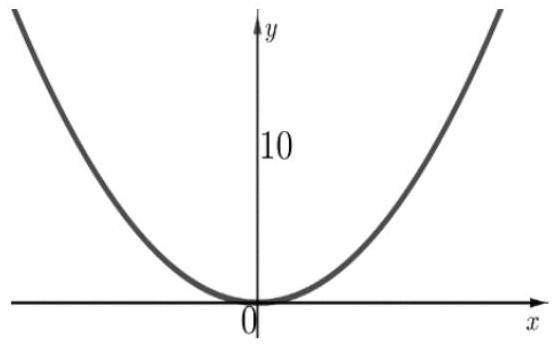
\includegraphics[max width=\textwidth, center]{ebe38402-76e9-4b46-a033-b1efc954d7e7-2_345_556_1165_1370}
  \item Proposition 3 : L'inéquation $4-7 x \leq 5 x-7$ a pour ensemble solution dans $\mathbb{R}$ :\\
a. $]-\infty ; \frac{11}{12}$ ]\\
b. $\left.]-\infty ;-\frac{11}{12}\right]$\\
c. $\left[\frac{11}{12} ;+\infty[\right.$\\
d. $\left[\frac{3}{2} ;+\infty[\right.$
  \item Proposition 4 : On considère une fonction $f$ définie sur $\mathbb{R}$ par $f(x)=5-9 x$
\end{enumerate}

Le tableau de signe de cette fonction est :\\
a.

\begin{center}
\begin{tabular}{|c|ccccc|}
\hline
$x$ & $-\infty$ &  & $\frac{5}{9}$ &  & $+\infty$ \\
\hline
$f(x)$ &  & - & 0 & + &  \\
\hline
\end{tabular}
\end{center}

c.

\begin{center}
\begin{tabular}{|c|ccccc|}
\hline
$x$ & $-\infty$ &  & $\frac{5}{9}$ &  & $+\infty$ \\
\hline
$f(x)$ &  & + & 0 & - &  \\
\hline
\end{tabular}
\end{center}

b.

\begin{center}
\begin{tabular}{|c|rrrrr|}
\hline
$x$ & $-\infty$ &  & $-\frac{5}{9}$ &  & $+\infty$ \\
\hline
$f(x)$ &  & - & 0 & + &  \\
\hline
\end{tabular}
\end{center}

d.

\begin{center}
\begin{tabular}{|c|rrrrr|}
\hline
$x$ & $-\infty$ &  & $-\frac{5}{9}$ &  & $+\infty$ \\
\hline
$f(x)$ &  & + & 0 & - &  \\
\hline
\end{tabular}
\end{center}

\section*{5. Proposition 5 : on a représenté ci-dessous une droite $\mathcal{D}$ dans un repère orthonormé.}
\begin{center}
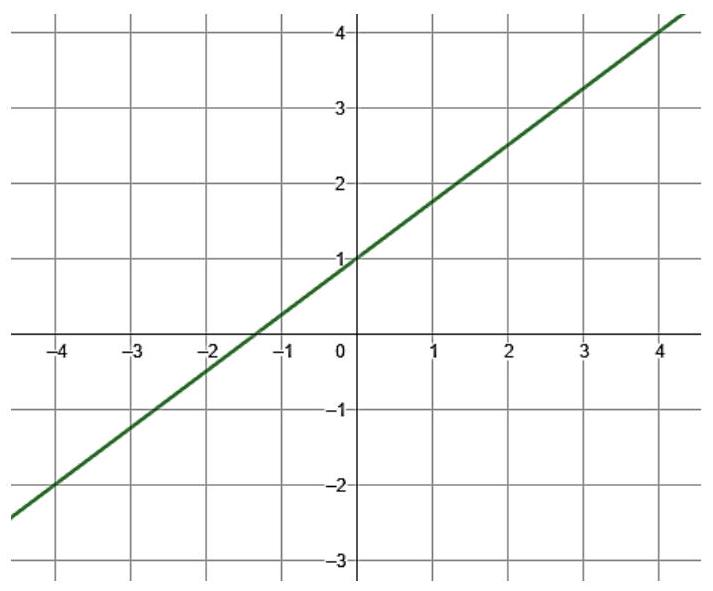
\includegraphics[max width=\textwidth]{ebe38402-76e9-4b46-a033-b1efc954d7e7-3_591_713_319_114}
\end{center}

Une équation de la droite $\mathcal{D}$ est :\\
a. $y=\frac{3}{4} x+1$\\
b. $y=\frac{4}{3} x+1$\\
c. $3 x-4 y+1=0$\\
d. $y=-\frac{3}{2} x+1$\\
6. Proposition 6 : On considère la fonction $f$ définie sur $\mathbb{R}$ par $f(x)=36 x^{2}-49$. La forme factorisée de $f(x)$ est:\\
a. $(6 x-7)^{2}$\\
b. $(36 x-49)(36 x+49)$\\
c. $36(x-7)^{2}$\\
d. $(6 x-7)(6 x+7)$

\section*{Exercice 2 \\
 (05 points)}
Un fermier souhaite réaliser un enclos rectangulaire pour des poules et des poussins, adossé à un mur de sa ferme afin d'économiser du grillage. Ainsi, il ne grillagera que 3 côtés de son enclos. Il possède 28 mètres de grillage. Il souhaite construire un enclos d'aire maximale. On appelle $x$ la longueur du côté de l'enclos perpendiculaire au mur.\\
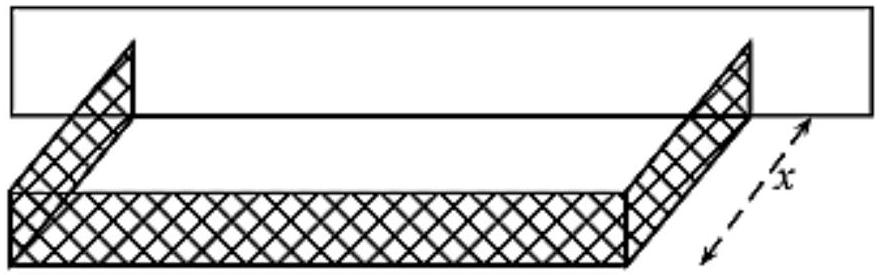
\includegraphics[max width=\textwidth, center]{ebe38402-76e9-4b46-a033-b1efc954d7e7-4_275_883_724_605}

On appelle $\mathcal{A}$ la fonction qui à un nombre $x$ associe $\mathcal{A}(x)$ l'aire de l'enclos.\\
La fonction $\mathcal{A}$ est ainsi définie sur l'intervalle [0;14].

\begin{enumerate}
  \item a. Vérifier que l'aire $\mathcal{A}(x)=-2 x^{2}+28 x$.\\
b. Montrer que la forme canonique de $\mathcal{A}(x)$ est $-2(x-7)^{2}+98$.
  \item Quatre courbes ont été tracées sur le graphique ci-dessous. Identifier celle qui représente la fonction $\mathcal{A}$.\\
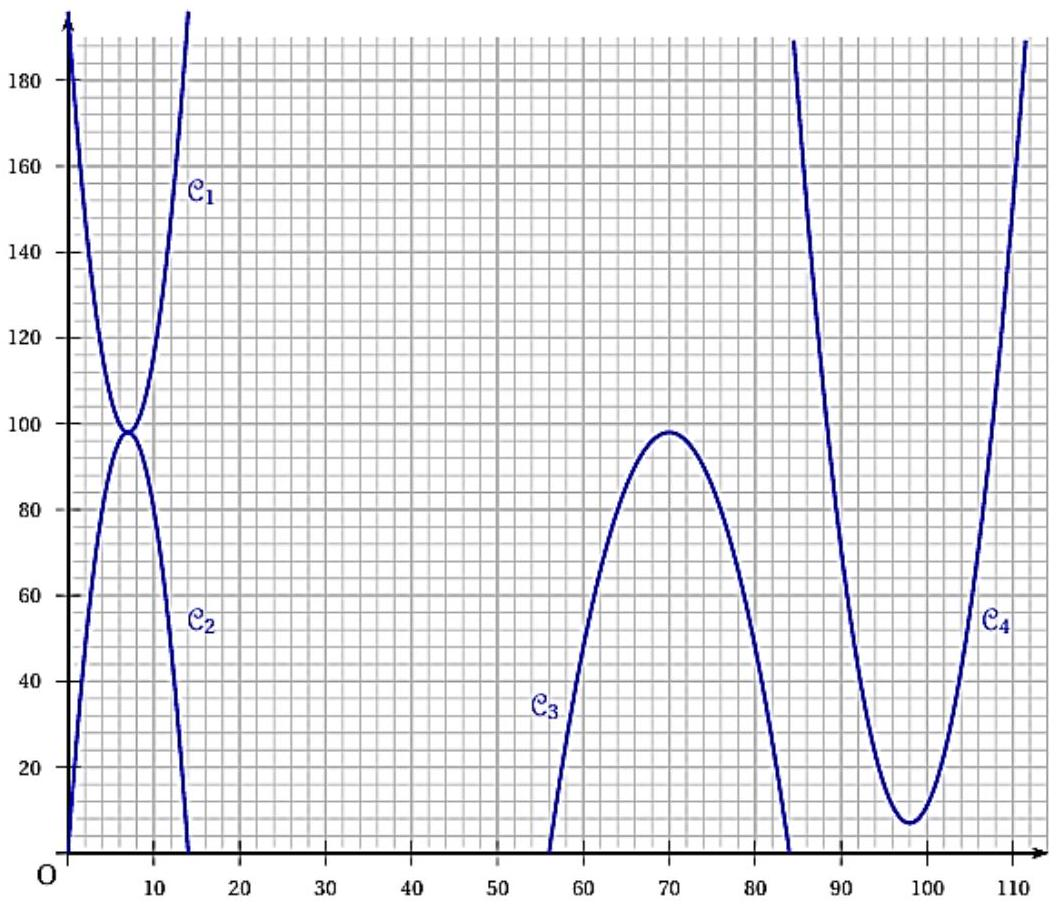
\includegraphics[max width=\textwidth, center]{ebe38402-76e9-4b46-a033-b1efc954d7e7-4_906_1056_1491_502}
  \item Dresser le tableau de variations de la fonction $\mathcal{A}$.
  \item Pour quelle valeur de $x$ l'aire de l'enclos est-elle maximale ? Donner la valeur de cette aire.
  \item Pour quelles valeurs de $x$ l'aire de l'enclos est-elle supérieure ou égale à $90 \mathrm{~m}^{2}$ ?
\end{enumerate}

\section*{Exercice 3 \\
 (04 points)}
On considère la fonction $f$ définie sur $[0 ; 5 \pi]$ par $f(x)=2 \cos \left(\frac{x+\pi}{2}\right)$.\\
La courbe représentative $\left(\mathcal{C}_{f}\right)$ de la fonction $f$ est représentée dans le repère ci-dessous:\\
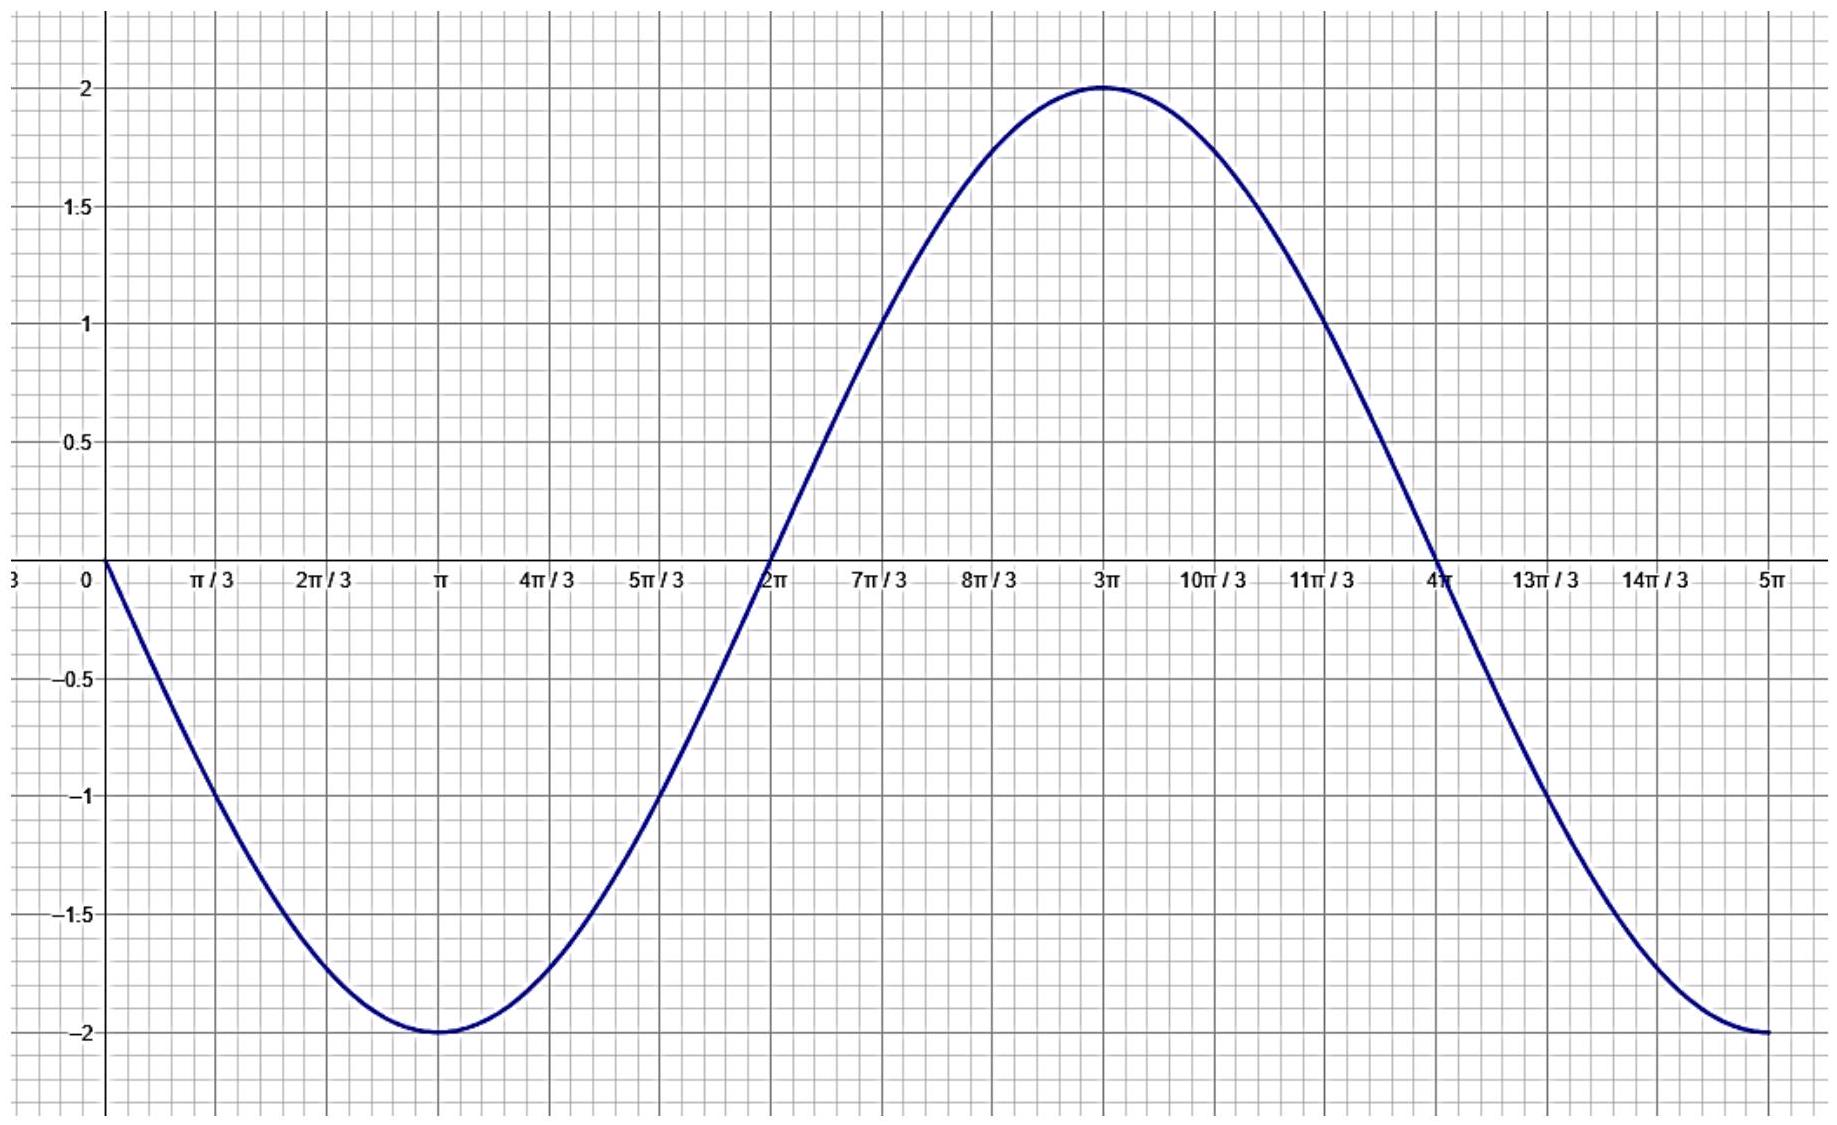
\includegraphics[max width=\textwidth, center]{ebe38402-76e9-4b46-a033-b1efc954d7e7-5_1125_1837_559_114}

\section*{Partie A: lectures graphiques}
Avec la précision permise par le graphique,

\begin{enumerate}
  \item Déterminer l'encadrement le plus précis possible de $f(x)$.
  \item Déterminer l'image de $\frac{13 \pi}{3}$ par la fonction $f$.
  \item Déterminer le(s) antécédent(s) de 1 par la fonction $f$.
\end{enumerate}

\section*{Partie B : justifications mathématiques}
\begin{enumerate}
  \item Démontrer que, pour tout $x$ de l'intervalle $[0 ; 5 \pi]$, on a $-2 \leq f(x) \leq 2$.
  \item a. Déterminer, en expliquant votre démarche, la mesure principale de $\frac{8 \pi}{3}$.\\
b. En déduire la valeur exacte de $f\left(\frac{13 \pi}{3}\right)$.
  \item a. En s'appuyant sur un cercle trigonométrique, résoudre l'équation $\cos (X)=\frac{1}{2}$ dans l'intervalle $\left[\frac{3 \pi}{2} ; \frac{5 \pi}{2}\right]$
  \item b. En déduire les solutions de l'équation $f(x)=1$ dans l'intervalle $[0 ; 5 \pi]$.
\end{enumerate}

\section*{Exercice 4 \\
 (05 points)}
Dans le plan muni d'un repère orthonormé ( $O ; \vec{\imath}, \vec{\jmath}$ ), on considère les points $A(5 ; 1), B(1 ; 4)$ et $C(2 ;-3)$.

Données : $\sqrt{50}=5 \sqrt{2}$ et $\frac{1}{\sqrt{2}}=\frac{\sqrt{2}}{2}$

\begin{enumerate}
  \item Tracer le triangle $A B C$ dans le repère donné ci-dessous :\\
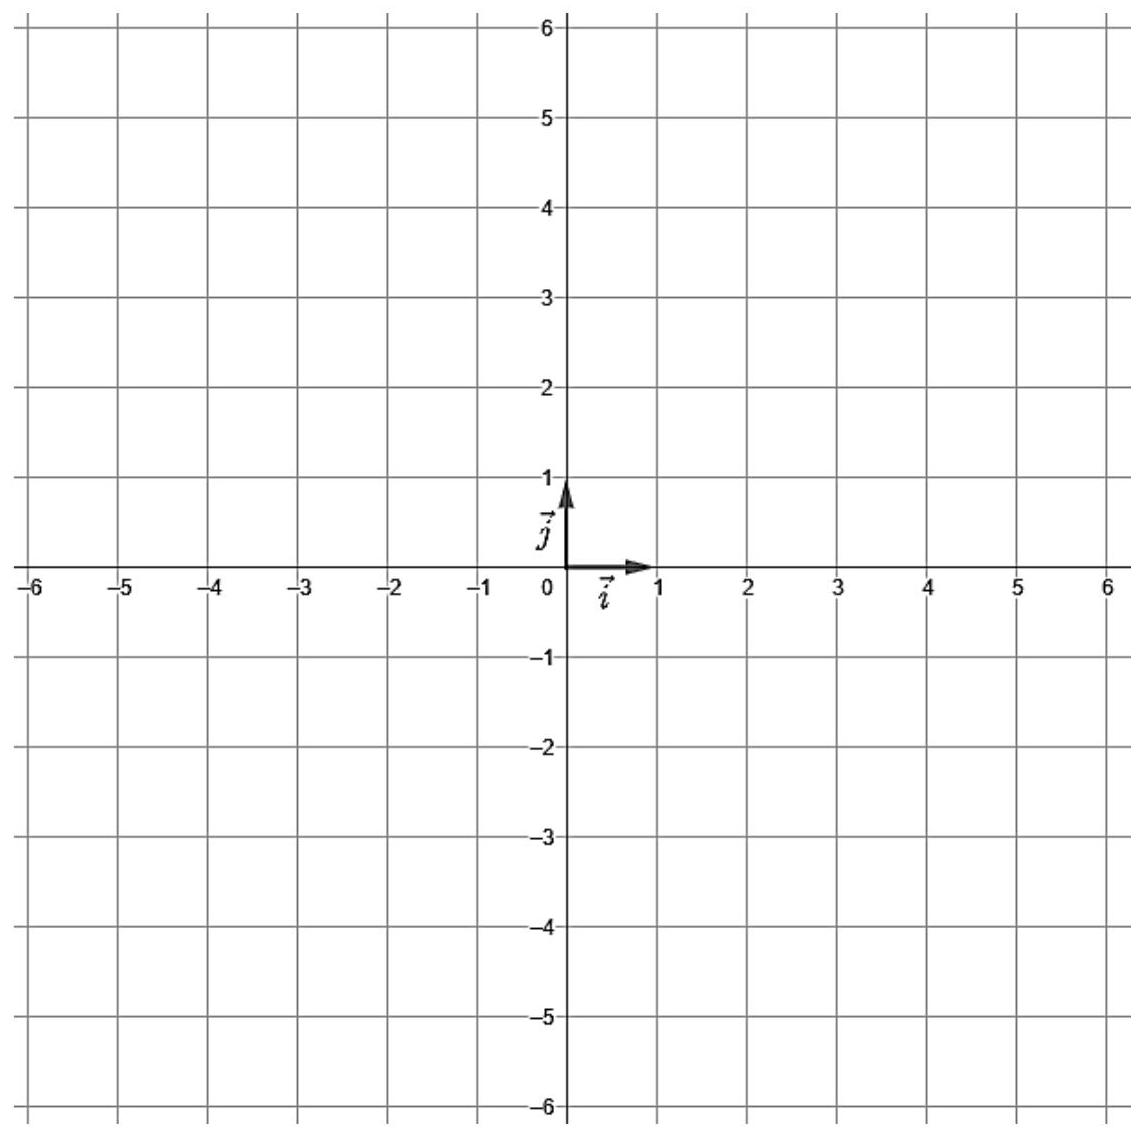
\includegraphics[max width=\textwidth, center]{ebe38402-76e9-4b46-a033-b1efc954d7e7-6_1137_1143_794_461}
  \item Calculer le produit scalaire $\overrightarrow{B C} \cdot \overrightarrow{B A}$.
  \item a. Exprimer $\overrightarrow{B C} \cdot \overrightarrow{B A}$ en fonction de l'angle ( $\overrightarrow{B C} ; \overrightarrow{B A}$ ).\\
b. En déduire la valeur exacte de l'angle orienté ( $\overrightarrow{B C} ; \overrightarrow{B A}$ ) en radians.
  \item Montrer que le triangle $A B C$ est rectangle, et préciser en quel point.
  \item a. Calculer les longueurs $A B$ et $A C$.\\
b. En déduire la valeur exacte de l'angle orienté $(\overrightarrow{C B} ; \overrightarrow{C A})$ en radians.
\end{enumerate}

\end{document}